\documentclass[11pt]{article}
\usepackage[final]{acl}
\usepackage{times}
\usepackage{latexsym}
\usepackage[T1]{fontenc}
\usepackage[utf8]{inputenc}
\usepackage{microtype}
\usepackage{inconsolata}
\usepackage{graphicx}
\usepackage{booktabs}
\usepackage{amsmath}

% DRAFT 2026-11-22. Every number below is taken from docs/EXPERIMENTS.md (recomputed from stored runs).
% TODO markers = items to confirm or experiments still missing (docs/EXPERIMENTS.md, section D).

\title{Do LLM Waypoints Help Heuristic Search?\\Reproducing LLM-A* and Rethinking Its Prompts}

\author{TODO Author \\
  Sungkyunkwan University \\
  \texttt{TODO@skku.edu}}

\begin{document}
\maketitle

\begin{abstract}
LLM-A* augments A* with waypoints proposed by a large language model (LLM).
We reproduce its main table with Llama-3-8B (operation ratio 45.55 vs.\ 44.59 reported) and extend it to GPT-4o mini, the backbone used for evaluation in this course.
A controlled analysis shows that the released search degenerates to weighted A* ($w{=}2$) when no waypoint survives filtering, and that this LLM-free variant needs fewer expansions (34.3) than LLM-A* with any released prompt on either model (45.6--64.0).
We then study prompt-side remedies and propose \emph{RePE2}, a one-call prompt that asks the model to try $0,1,2,\dots$ waypoints in rounds and to stop at the first round it judges collision-free.
On 1{,}000 problems RePE2 lowers the operation ratio of GPT-4o mini LLM-A* to 40.1, a paired 17--25\% reduction over the released prompts, and cuts runaway searches from 49--67 to 14; an ablation attributes the gain to the round procedure rather than to the demonstrations, and the gain carries over to four of five unseen map families.
Re-running all stored responses through stronger searches with matched no-LLM controls shows that GPT-4o mini waypoints add little, except in an experience-graph search that keeps only collision-free segments, where a barrier-end candidate prompt yields a 12\% reduction.
The model's self-checks are almost always wrong (97\% of ``valid'' verdicts), locating the bottleneck in its collision reasoning.
\end{abstract}

\section{Introduction}
Path planning on grid maps is a classic search problem: A* \citep{hart1968astar} returns optimal paths but may expand many states.
LLM-A* \citep{meng2024llmastar} asks an LLM for a coarse list of waypoints and uses them as moving targets inside A*, reporting fewer operations and less storage than A* on 1{,}000 problems.
This assignment asks us to reproduce the main table and to propose an improved algorithm that keeps the baseline input/output format and is evaluated with GPT-4o mini on hidden maps.

Our study proceeds in three steps.
(i) We reproduce Table~1 with Llama-3-8B and extend it to GPT-4o mini (\S\ref{sec:repro}).
(ii) We diagnose where the gain of LLM-A* comes from and find that LLM waypoints are, on average, harmful under the released search (\S\ref{sec:diag}).
(iii) We test prompt-side and search-side remedies, propose RePE2, and quantify how much LLM waypoints contribute once the search itself is improved (\S\ref{sec:results}).

\paragraph{Contributions.}
(1) A verified reproduction (4{,}000 paths match the released implementation) plus a GPT-4o mini extension.
(2) A diagnosis with matched no-LLM controls showing that the released LLM-A* is dominated by weighted A* with the same formula and no waypoints.
(3) RePE2, a one-call prompt that significantly reduces search effort of GPT-4o mini LLM-A* (operation ratio 53.2/49.9/48.4 $\rightarrow$ 40.1).
(4) A controlled analysis of post-inference search: GPT-4o mini waypoints add almost nothing under improved LLM-A* variants or a geometric heuristic, but give a significant 12\% gain when an experience-graph search uses only their collision-free segments; we document failure modes and the gap to an oracle.

\section{Related Work}
\paragraph{Heuristic search.}
Weighted A* \citep{pohl1970weighted} inflates the heuristic to trade optimality for speed; the maximum of admissible heuristics is admissible \citep{pearl1984heuristics}.
Experience Graphs \citep{phillips2012egraphs} and Multi-Heuristic A* \citep{aine2016mha} use external guidance with bounded suboptimality.
Visibility graphs \citep{lozano1979visibility} and subgoal graphs \citep{uras2013subgoal} exploit obstacle corners, which inspires our geometric baseline.
\paragraph{LLMs for planning and prompting.}
LLM-A* \citep{meng2024llmastar} injects LLM waypoints into A* with few-shot, chain-of-thought \citep{wei2022cot} and recursive path evaluation (RePE) prompts.
Visualization-of-Thought \citep{wu2024vot} elicits spatial reasoning by drawing intermediate states.
Least-to-most decomposition \citep{zhou2023leasttomost} and self-refinement \citep{madaan2023selfrefine} motivate our round-based prompt, while LLM self-verification is known to be unreliable \citep{huang2024selfcorrect}, which our results confirm.

\section{Task and Baseline}
\label{sec:repro}
\paragraph{Data and metrics.}
We use the released dataset: 100 maps of size $51\times31$ with axis-aligned barriers, 10 start/goal pairs each.
Following the paper, for every problem we divide the number of heap pops (\emph{operation}, duplicates included as in the released code), the size of the cost table (\emph{storage}) and the path length by those of A*, and report the geometric mean $\times100$ (lower is better).
\paragraph{LLM-A*.}
The released search expands $f(s)=g(s)+h(s,\text{goal})+h(s,t_k)$ where $t_k$ is the current waypoint; it switches to the next waypoint when a neighbour equals $t_k$, and drops waypoints on barriers or near the border before search.
If every waypoint is dropped, $f=g+2h$, i.e.\ weighted A* with $w{=}2$.
\paragraph{Reproduction setup.}
Llama-3-8B-Instruct (fixed revision, bf16, greedy decoding, 8{,}000 new tokens) with the released prompts; our implementation reproduces the released search exactly on 4{,}000 stored paths.
For GPT-4o mini (\texttt{gpt-4o-mini-2024-07-18}, temperature 0, 8{,}000 tokens, Batch API) we keep the released GPT prompts.
This is an extension, not a reproduction of the paper's GPT-3.5 row: the paper used a completion model with a 100-token, newline-stopped output.

\begin{table}[t]
\centering\small
\setlength{\tabcolsep}{3.5pt}
\begin{tabular}{llccc}
\toprule
Model & Prompt & Op. & Stor. & Len. \\
\midrule
Llama-3 (paper) & Few-shot & 44.59 & 64.02 & 102.47 \\
Llama-3 (ours) & Few-shot & 45.55 & 64.78 & 102.55 \\
Llama-3 (paper) & CoT & 47.60 & 66.27 & 102.46 \\
Llama-3 (ours) & CoT & 48.04 & 66.73 & 102.52 \\
Llama-3 (paper) & RePE & 64.08 & 80.19 & 102.54 \\
Llama-3 (ours) & RePE & 63.95 & 80.14 & 102.60 \\
\midrule
GPT-4o mini & Few-shot & 49.96 & 68.10 & 102.95 \\
GPT-4o mini & CoT & 48.41 & 67.08 & 102.63 \\
GPT-4o mini & RePE & 53.24 & 70.51 & 102.54 \\
\midrule
Weighted A* $w{=}2$ & -- & 34.32 & 56.23 & 102.02 \\
\bottomrule
\end{tabular}
\caption{LLM-A* reproduction (1{,}000 problems, \% of A*). Weighted A* equals LLM-A* with all waypoints removed.}
\label{tab:repro}
\end{table}

\section{Diagnosis: Where Does the Gain Come From?}
\label{sec:diag}
Table~\ref{tab:repro} already shows the central issue: the LLM-free special case of the released formula, weighted A* ($w{=}2$), expands fewer states than LLM-A* with every prompt and both models, at a shorter path.
Paired against this control, GPT-4o mini waypoints increase operations by 41--55\% (Table~\ref{tab:post}, column ``official'').
Three further observations (Llama-3 responses, offline) point to the waypoints themselves.
One random waypoint drawn inside the start--goal rectangle gives an operation ratio of 39.8 (two: 45.3), lower than LLM-A* with any released Llama-3 prompt (45.6--64.0);
the LLM picks the correct side around the first blocking wall less often (77.2\%) than a trivial ``shorter detour'' rule (86.4\%);
and the waypoint-based distance has near-zero rank correlation with the true cost-to-go (0.75 for oracle waypoints).
Failure modes visible in the responses are waypoints placed on barriers, segments that cut barrier corners, and long detour chains that the target-switching rule follows even after they have been passed.

\section{Method: RePE2}
\label{sec:method}
Our prompt-side study (\S\ref{sec:results}) suggested that the costly failures are \emph{too many and detouring} waypoints rather than slightly invalid ones.
RePE2 therefore asks for the fewest waypoints first.
The released instruction is kept and one sentence is added: \emph{``Find the path in rounds. Round $k$ uses exactly $k$ intermediate waypoints, starting from Round 0 (a straight line from the start to the goal). After each round, check whether every segment avoids all barriers, and stop at the first valid round.''}
Each of five demonstrations shows the rounds, a one-line check per round, and the final \texttt{Generated Path}; the output format and parser are unchanged, so the search and the I/O format of the baseline are untouched and the prompt runs in a single call.
\paragraph{Demonstrations.}
The released demonstrations are unrepresentative of the evaluation set: 2 of 5 are solvable by a straight line (0.6\% of evaluation problems) and 3 of 5 use more waypoints than necessary.
We therefore generated new $51\times31$ maps \emph{outside the evaluation set} with barrier counts and lengths sampled from the dataset, computed for each problem the exact minimum number of waypoints over all cells the released filter keeps, and selected one problem each with minimum 0, 2, 1, 3 and 1 waypoints (the 1-waypoint case covers 88\% of evaluation problems).
Among dataset-like candidates (5--7 barriers, a real detour) we picked those whose shortest minimal chain gives the lowest LLM-A* operation ratio.
Every round and verdict in the demonstrations is verified against the exact segment--barrier intersection test.

\section{Experiments}
\label{sec:results}
\paragraph{Prompt-side variants.}
All variants keep the released search and are run on the full 1{,}000 problems with GPT-4o mini unless noted.
Waypoint cap (``use at most $N$ waypoints'', $N$ = number of barriers): 48.5/49.6/53.0, no change; the same cap on Llama-3 also had no clear effect.
Zero-shot Visualization-of-Thought trigger plus cap: 52.5, with 98 truncated outputs and 294 cell-by-cell walks; adding an ASCII map (10-problem pilots) led the model to copy the grid or swap axes, so we did not pursue a true visual variant.
Listing the cells just beyond each barrier end as candidate waypoints raised the LLM-only success rate from 6.5\% to 34.7\% (Few-shot) and helped RePE (53.2$\rightarrow$46.9, paired 88.1\% [83.4, 92.7]) but not Few-shot or CoT, because the model chained unnecessary candidates into detours (chains $\geq1.6\times$ the optimal length: 18$\rightarrow$148).

\begin{table}[t]
\centering\small
\setlength{\tabcolsep}{3pt}
\begin{tabular}{lccc}
\toprule
Prompt (GPT-4o mini) & Op. & RePE2 / prompt & $>2\times$A* \\
\midrule
Few-shot & 49.96 & 80.3 [76.7, 83.9] & 52 \\
CoT & 48.41 & 82.9 [79.2, 86.7] & 49 \\
RePE & 53.24 & 75.3 [71.8, 78.9] & 67 \\
Endpoint list + RePE & 46.89 & 85.6 [81.8, 89.5] & 37 \\
\textbf{RePE2 (ours)} & \textbf{40.12} & -- & \textbf{14} \\
\quad new demos, no rounds & 51.15 & 78.4 [74.8, 82.2] & 60 \\
\quad released demos + rounds & 40.27 & 99.6 [96.9, 102.4] & 11 \\
\midrule
Weighted A* $w{=}2$ & 34.32 & 116.9 [114.0, 120.3] & 3 \\
\bottomrule
\end{tabular}
\caption{RePE2 vs.\ prompts on 1{,}000 problems. Middle column: paired ratio of operations (geometric mean, bootstrap 95\% CI over problems). Last column: problems with more than twice the operations of A*.}
\label{tab:repe2}
\end{table}

\paragraph{RePE2.}
Table~\ref{tab:repe2} shows that RePE2 reduces operations significantly against every released prompt (storage 61.0 vs.\ 67.1--70.5; path length 102.4, unchanged) and makes runaway searches rare.
Outputs are short (294 tokens on average) and never truncated.
The number of waypoints it returns (0:86, 1:609, 2:201, 3:96, $\geq$4:8) resembles the number of turning points of optimal paths (0:6, 1:774, 2:176, 3:40, $\geq$4:4).
\paragraph{Ablation.}
Two further runs separate the new demonstrations from the round procedure.
The new demonstrations in the plain Few-shot format (no rounds, no added sentence) give 51.15, no better than the released Few-shot prompt (paired 102.4\% [97.7, 107.7]).
The released demonstrations rewritten in the round format, with the added sentence, give 40.27, indistinguishable from RePE2 (100.4\% [97.7, 103.2]).
The gain therefore comes from the round procedure, not from the choice of demonstrations.

\paragraph{The self-check does not work.}
Over 2{,}517 parsed rounds, the model's ``Not valid'' verdicts are almost always right (1{,}507 of 1{,}521) but its ``Valid'' verdicts are almost always wrong (968 of 996).
Only 2.8\% of final paths are collision-free, and a round that follows a ``Not valid'' verdict actually removes the collision in 2.4\% of cases.
Although 72\% of the failing paths cross a single barrier, moving one waypoint by one cell repairs only 7\% of them: the path passes the wrong side of a barrier rather than narrowly grazing it.
RePE2 helps because its waypoints are few and close to the straight line, so the released target-switching rule is rarely misled, not because they are correct.
It still does not beat the LLM-free weighted A*.

\begin{figure}[t]
\centering
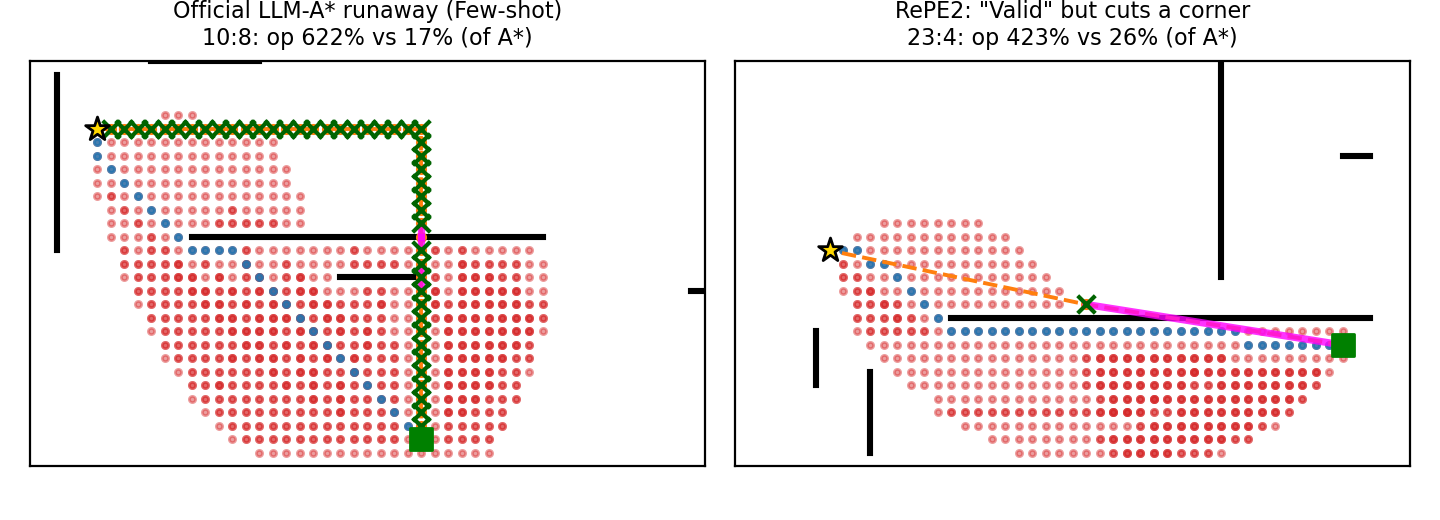
\includegraphics[width=\columnwidth]{fig_failures.png}
\caption{Failure cases (picked by rule: largest LLM-A*/weighted-A* ratio). Left: released Few-shot prompt, cell-by-cell waypoints crossing a barrier; LLM-A* (red) expands 983 states, weighted A* (blue) 27. Right: RePE2 answer declared ``Valid'' whose segment (magenta) crosses a barrier.}
\label{fig:fail}
\end{figure}

\paragraph{Improving the search instead.}
We re-ran every stored GPT-4o mini response through three modified searches and compared each with the same search given no waypoints (Table~\ref{tab:post}).
\emph{Progress switching} drops a waypoint once the current node is closer to the goal than the waypoint;
\emph{+weights} additionally scales the goal term by 2 and the waypoint term by 0.5;
\emph{wallC+route} replaces the heuristic by $1.5\max(h_{C}(s), h_{R}(s))$, where $h_{C}$ is the shortest detour around the convex hulls of connected barrier groups crossed by the segment to the goal (admissible, computed in closed form per node) and $h_{R}$ follows the LLM chain, used only if every chain segment is collision-free.

\begin{table}[t]
\centering\small
\setlength{\tabcolsep}{2.6pt}
\begin{tabular}{lcccc}
\toprule
Responses & official & progress & +weights & wallC+route \\
\midrule
no waypoints & 34.32 & 34.32 & 31.60 & 15.44 \\
Few-shot & 49.96 & 37.90 & 32.56 & 15.42 \\
Endpoint Few-shot & 52.50 & 34.49 & 31.37 & 15.05 \\
RePE2 & 40.12 & 37.15 & 32.57 & 15.44 \\
\midrule
LLM / no-LLM & 137--155 & 100--113 & 99--104 & 97--100 \\
\bottomrule
\end{tabular}
\caption{Operation ratio of modified searches on stored GPT-4o mini responses (1{,}000 problems). Last row: range of paired ratios over all ten response sets (original, capped, endpoint and RePE2 prompts).}
\label{tab:post}
\end{table}

Better search removes the harm of LLM waypoints but leaves almost no benefit: across all response sets the paired ratio to the matched no-LLM control is 99--104\% with weights and 97--100\% with wallC.

\paragraph{Collision-free experience helps.}
Experience-graph search \citep{phillips2012egraphs} uses only the collision-free segments of the LLM path as cheap ``experience'' and keeps a suboptimality bound ($\le w\varepsilon_E$).
With $\varepsilon_E{=}1.5$, $w{=}1.33$ (duplicate pops skipped, as is standard for this algorithm), the endpoint-list Few-shot responses---which have the highest collision-free rate (34.7\%)---reduce operations to 30.24 (length 102.85) against 34.52 without waypoints, a paired 87.6\% [85.6, 89.5] that holds on both halves of the maps (88.1\% / 87.1\%) and lies below the weighted A* trade-off curve (32.2 at length 103.0).
This is the only setting in which GPT-4o mini waypoints give a clear net gain.
RePE2 responses, almost never collision-free, hurt in this search (108.3\%), so the best prompt depends on how the search uses the waypoints.
Oracle waypoints reach 21.8 in the same search.
The geometric heuristic alone reaches 15.4 (path length 100.15, no invalid path), and with \emph{oracle} waypoints (turning points of the optimal path) the same search reaches 12.1, an upper bound on what a perfect LLM could add.
Operations do not include heuristic cost: with collisions checked on demand as in the released code, wallC takes 3.05\,ms per search against 2.76\,ms for weighted A* on these maps, and is faster only on larger maps.

\paragraph{Other map families.}
To probe generalisation to unseen maps we ran the same prompts, unchanged, on 500 generated problems from five families (100 each): dense barriers, rooms with narrow doors, U-shaped traps, mazes, and the original layout scaled to $101\times61$.
RePE2 again lowers LLM-A* operations against the Few-shot prompt (overall 53.9$\rightarrow$38.5, paired 71.3\% [66.6, 76.1]; 63--71\% in four families), but not in mazes (96.0\% [88.6, 103.8]), where optimal paths turn 6.6 times on average and RePE2 returns only 2.2 waypoints: asking for the fewest waypoints first under-supplies them.
It remains worse than weighted A* in every family (overall 112.6\%).
The endpoint prompt with experience graphs still reduces operations against the no-waypoint control (overall 93.3\% [90.7, 95.8]; rooms 92.5\%, U-traps 96.5\%, scaled 80.0\%; no effect on dense maps).
The geometric heuristic is lowest in all families (overall 23.0 vs.\ 34.2 for weighted A*).

\paragraph{Where failures come from.}
Classifying every response shows that even collision-free LLM paths cost more than weighted A* under the released search (Few-shot: 29 vs.\ 21 on the same problems), because they often follow long axis-aligned routes that the waypoint term then enforces; a perfect choice among barrier-end cells bounds the released search at 31.3.
Problems that need two or more waypoints are hard for every prompt (63--89 vs.\ 58--59 for weighted A*).
Figure~\ref{fig:fail} shows two representative failures.

\section{Conclusion}
We reproduced LLM-A* and showed, with matched controls, that its released form is dominated by the weighted A* hidden in its own formula.
Among prompt-side remedies, RePE2 gives the largest and statistically clear improvement for GPT-4o mini (40.1 vs.\ 48.4--53.2) while keeping the baseline search and I/O format, and the gain comes from asking for the fewest waypoints first.
Our analyses locate the bottleneck in the LLM's geometric verification: it recognises blocked straight lines but cannot check its own repairs.
LLM waypoints pay off only when the search consumes their collision-free parts (experience graphs, 12\% gain), which suggests combining prompts that raise the collision-free rate with searches that ignore the rest.
Future work should give the model verifiable feedback (collision reports between rounds) and test on other map families.

\section*{Limitations}
The main results use the released dataset of small maps; the five generated families cover only 100 problems each. All runs use greedy decoding without repetition.
Search variants and thresholds were explored on the same data (direction checked on a split of maps); the experience-graph parameters were chosen on Llama-3 responses.
RePE2 demonstrations were selected by the evaluation metric on separate synthetic maps, although the ablation shows they do not drive the gain; the round instruction and the round-format demonstrations were not separated.
The experience-graph result is offline and not yet the default path of the submitted code.
Operation counts ignore heuristic computation; the geometric heuristic is slower in wall-clock time than weighted A*.
The GPT-4o mini runs extend rather than reproduce the paper's GPT-3.5 setting.
% TODO: individual contribution report is submitted separately.

\bibliography{custom}

\appendix
\section{Reproducibility}
All configurations, prompts, stored responses, analysis scripts and tests are in the code archive; \texttt{docs/EXPERIMENTS.md} lists every run and \texttt{docs/RUNS.md} maps runs to configurations and scripts.

\end{document}
